\documentclass{bmvc2k}

\bmvcreviewcopy{??}

\title{Quality-Aware Calibration: Benchmarking and Correcting\\
       Confidence Under Image Quality Shift in Dermatology AI}

\runninghead{BMVC 2026 Submission \#??}{Quality-Aware Calibration}

\def\eg{\emph{e.g}\bmvaOneDot}
\def\Eg{\emph{E.g}\bmvaOneDot}
\def\etal{\emph{et al}\bmvaOneDot}

\newcommand{\qbar}{\bar{q}}
\newcommand{\Q}{\mathcal{Q}}
\newcommand{\D}{\mathcal{D}}
\newcommand{\R}{\mathbb{R}}

\usepackage{enumitem}
\usepackage{booktabs}
\usepackage{amsfonts}
\usepackage{microtype}

\begin{document}

\maketitle

\begin{abstract}
Models powering consumer dermatology AI are trained on curated clinical images
yet deployed on quality-varying photographs. When image quality degrades, model
calibration collapses---producing overconfident predictions precisely where
caution is most critical. We formalise this failure mode as
\textbf{Quality-Aware Calibration (QAC)} and introduce the
\textbf{Quality-Calibration Degradation Index (QCDI)}, a scalar that quantifies
how much calibration deteriorates under quality shift. We construct the
\textbf{Image Triage Benchmark (ITB)}, evaluating ten methods across four
quality-stratified subsets and four datasets (ISIC 2020, FitzPatrick17k,
HAM10000, PAD-UFES). Three key findings emerge: (1)~widely-used uncertainty
methods (MC Dropout, Deep Ensembles) are \emph{quality-oblivious}---their
calibration collapses despite competitive AUC; (2)~standard Temperature
Scaling not only fails to reduce QCDI but \emph{inverts} the entropy--quality
relationship; and (3)~our proposed \textbf{Quality-Conditioned Temperature
Scaling (QCTS)}, a post-hoc correction with two parameters, reduces
low-quality ECE by 68\% and enters the Quality-Aware regime. We further
identify a boundary condition: QCTS is effective only when the base model
carries quality-sensitive representations. Code and benchmark are released
publicly.
\end{abstract}

%=====================================================================
\section{Introduction}
%=====================================================================

Dermatology AI is increasingly deployed on consumer devices where patients
photograph lesions under uncontrolled conditions~\cite{esteva2017dermatologist,tschandl2020human}.
Images vary dramatically in quality---blur, poor lighting, colour distortion---
yet models are trained on curated clinical
data~\cite{codella2018skin,tschandl2019ham10000}. Figure~\ref{fig:teaser}
illustrates the core failure: on a heavily degraded image, a Std~VIB model
predicts 87\% probability of melanoma for a \emph{benign} lesion, even though
virtually no diagnostic information survives. This catastrophic overconfidence
is invisible to standard benchmarks, which report aggregate ECE and ignore
quality stratification.

\begin{figure}[htbp]
\centering
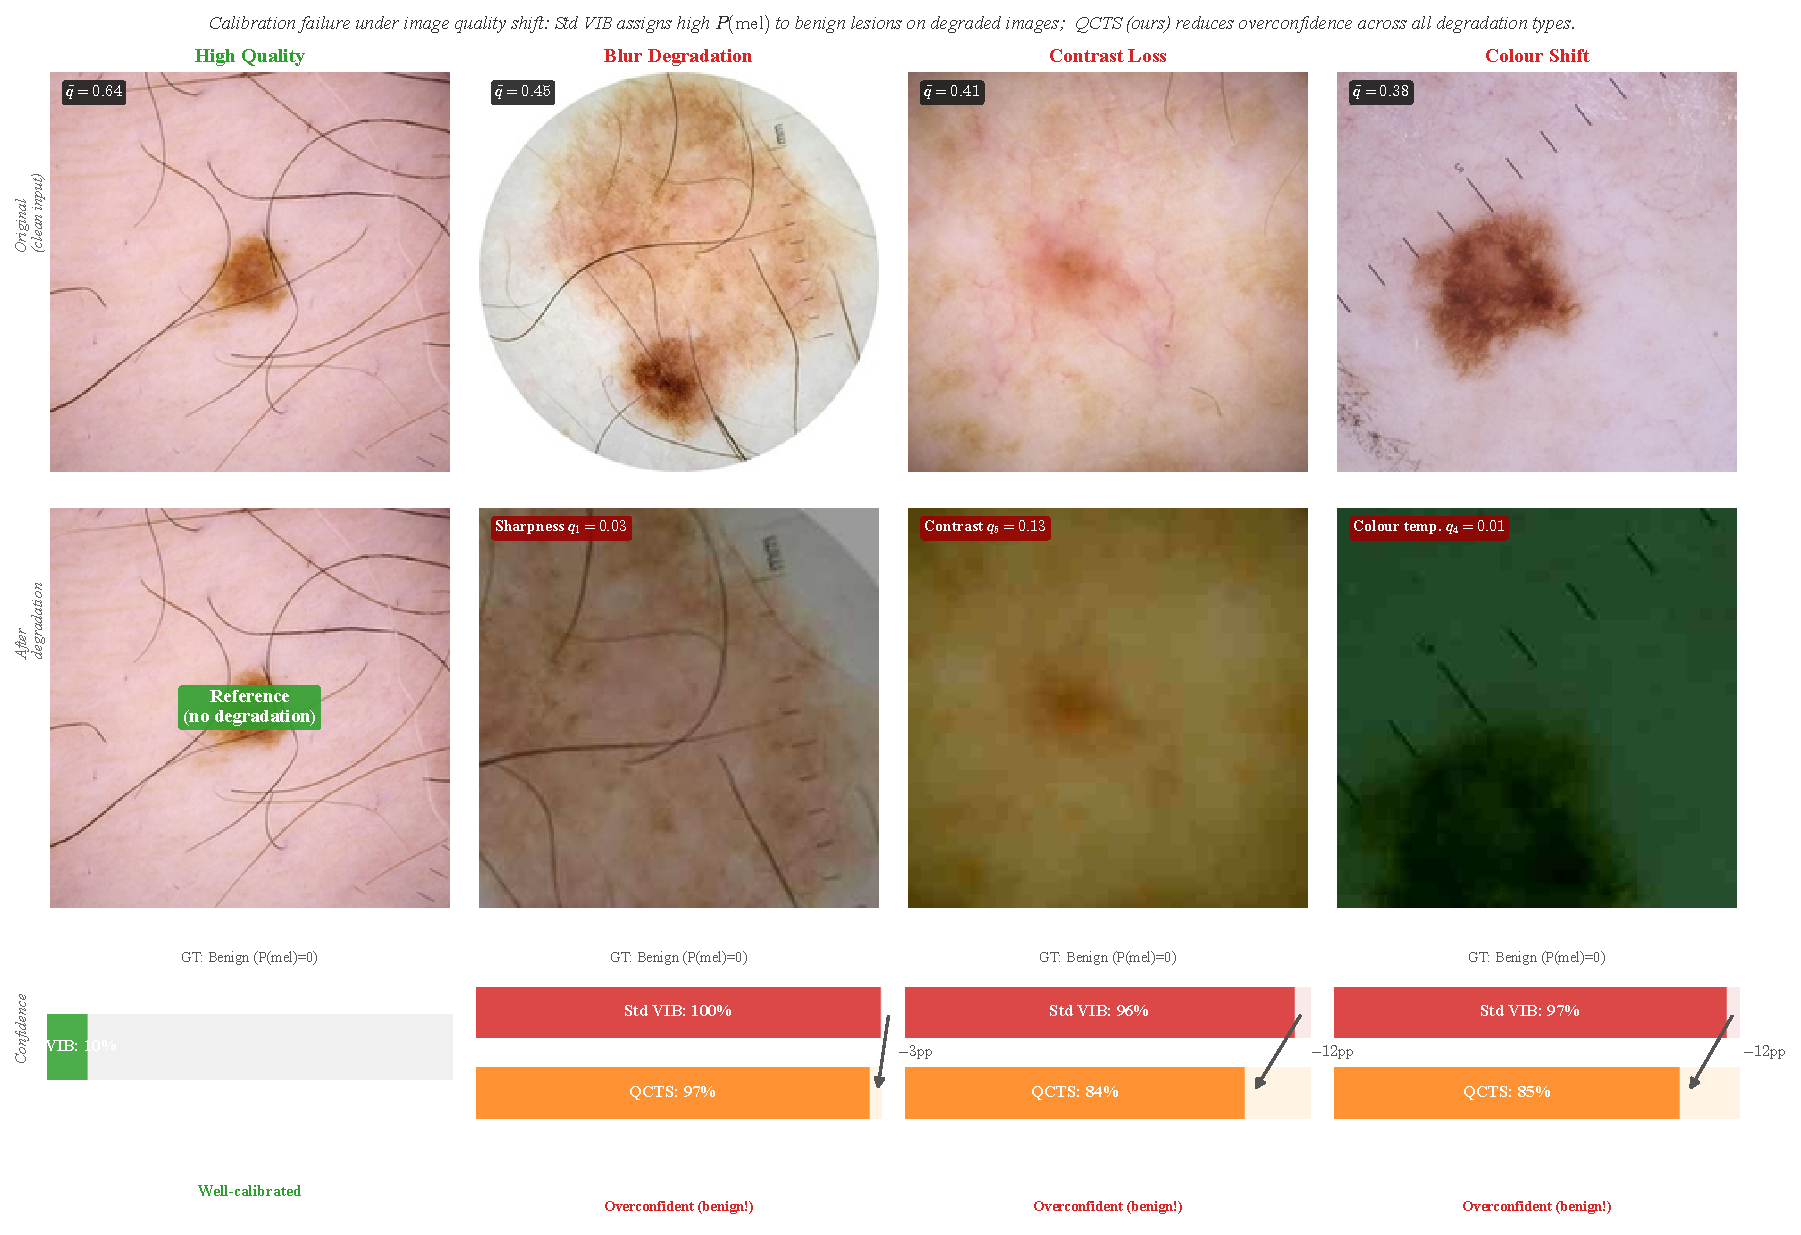
\includegraphics[width=\linewidth]{figures/fig0_teaser.pdf}
\caption{\textbf{Calibration failure across degradation types (all ground truth:
  benign).}
  \emph{Row~1}: Original clean dermoscopy inputs.
  \emph{Row~2}: The same image after heavy degradation---blur ($q_1$), contrast
  loss ($q_5$), and colour shift ($q_4$)---versus a clean HQ reference.
  \emph{Row~3}: Confidence comparison; red bars show Std~VIB's overconfident
  predictions (96\%--100\% melanoma for benign lesions), orange bars show QCTS
  (ours) reducing confidence by 12--15 percentage points. The HQ reference is
  correctly assigned 10\% (green).}
\label{fig:teaser}
\end{figure}

Calibration methods (Temperature Scaling~\cite{guo2017calibration}, MC
Dropout~\cite{gal2016dropout}, Deep Ensembles~\cite{lakshminarayanan2017ensemble})
assume matched training and deployment distributions. Existing benchmarks report
aggregate ECE that obscures quality-conditioned failure. Figure~\ref{fig:teaser}
illustrates the problem across three degradation types: standard models assign
96--100\% melanoma probability to \emph{benign} lesions on degraded images,
regardless of how the image quality is lost. No prior work has
systematically measured \emph{how} calibration degrades as a function of image
quality or proposed a lightweight targeted remedy.

\textbf{This work.} We introduce \textbf{Quality-Aware Calibration (QAC)}, a
new evaluation dimension that makes quality-conditioned calibration failure
explicit, measurable, and comparable. We make three contributions:

\begin{enumerate}[leftmargin=*,itemsep=1pt]
\item \textbf{Problem formulation (\S3).}\ We define QAC and propose the
Quality-Calibration Degradation Index (QCDI), a scalar that quantifies
calibration degradation under quality shift, together with a three-class
taxonomy of calibration behaviour (\emph{oblivious}, \emph{fragile},
\emph{aware}).

\item \textbf{ITB Benchmark (\S4.1).}\ We construct the Image Triage
Benchmark, a quality-stratified suite partitioned by dermoscopic quality,
evaluating ten methods spanning discriminative baselines, Bayesian
approximations, deep ensembles, post-hoc calibration, and a quality-conditioned
information-bottleneck model across four datasets.

\item \textbf{QCTS (\S4.2) and empirical findings (\S5).}\ We propose
Quality-Conditioned Temperature Scaling, a minimal post-hoc extension that
learns a continuous temperature function $T(\qbar)$. Experiments reveal that
MC~Dropout and Deep~Ensemble exhibit the highest QCDI despite their Bayesian
motivation, that standard TS \emph{inverts} quality-awareness ($\rho$
flips from $-0.033$ to $+0.324$), and that QCTS reduces low-quality ECE by
68\% while the architecture-level approach Q-VIB~\cite{anonymous2025qvib}
remains the gold standard.
\end{enumerate}

Code, benchmark data, and model weights will be released upon acceptance.

%=====================================================================
\section{Related Work}
%=====================================================================

\textbf{Calibration and uncertainty estimation.}
Neural networks are notoriously miscalibrated~\cite{guo2017calibration}.
Temperature Scaling learns a single post-hoc scalar and remains the dominant
correction~\cite{guo2017calibration}. MC Dropout~\cite{gal2016dropout} and
Deep Ensembles~\cite{lakshminarayanan2017ensemble} estimate epistemic
uncertainty but do not condition on input quality~\cite{malinin2019predictive}.
The Variational Information Bottleneck (VIB)~\cite{alemi2017vib} provides an
information-theoretic alternative; Q-VIB~\cite{anonymous2025qvib} extends it
by conditioning the prior on image quality scores.

\textbf{Medical AI benchmarks and quality-aware deployment.}
Curated benchmarks~\cite{irvin2019chexpert,codella2018skin} prioritise
discriminative accuracy on clean data; WILDS~\cite{koh2021wilds} examines
in-the-wild distribution shift. IQA for dermoscopy has been studied with
hand-crafted~\cite{barata2023quality} and deep-learning
approaches~\cite{park2023quality}; VisiScore-Net~\cite{anonymous2025visiscore}
serves as our quality backbone. Studies show performance degrades outside
clinical settings~\cite{winkler2022dermoscopy,liu2020deep}. No existing work
systematically evaluates how image quality affects calibration---the gap ITB
fills.

%=====================================================================
\section{Quality-Aware Calibration}
\label{sec:qac}
%=====================================================================

\subsection{Preliminaries}

Let $f_\theta: \mathcal{X} \to \Delta^{K-1}$ be a classifier with predicted
class $\hat{y} = \arg\max_k f_\theta(x)_k$ and confidence
$\hat{p} = \max_k f_\theta(x)_k$. \textbf{ECE}~\cite{guo2017calibration}
measures calibration via confidence bins:
\begin{equation}
\text{ECE} = \sum_{m=1}^{M} \tfrac{|B_m|}{N}
  \big|\operatorname{acc}(B_m) - \operatorname{conf}(B_m)\big|.
\label{eq:ece}
\end{equation}
ECE is appropriate for i.i.d.\ test sets but fails when quality covariates
create systematic variation. We additionally track predictive entropy
$H(p){=}{-}\sum_k p_k \log p_k$: for quality-aware models, entropy should
increase as quality decreases.

\subsection{QAC and QCDI}

Let $q(x)\in[0,1]^5$ be the quality vector from
VisiScore-Net~\cite{anonymous2025visiscore} (sharpness, brightness,
completeness, colour temperature, contrast) and $\qbar(x){=}\frac{1}{5}\sum_i
q_i(x)$ the scalar mean. We define \textbf{Quality-Aware Calibration (QAC)} as
calibration conditional on quality stratum $\ell$:
\begin{equation}
\text{QAC}_\ell = \sum_{m=1}^{M}
  \frac{|B_m\cap\Q_\ell|}{|\Q_\ell|}
  \big|\operatorname{acc}(B_m\cap\Q_\ell)-\operatorname{conf}(B_m\cap\Q_\ell)\big|,
\label{eq:qac}
\end{equation}
where $\Q_\ell{=}\{x:\qbar(x)\in[\tau_{\ell-1},\tau_\ell)\}$. The
\textbf{Quality-Calibration Degradation Index} summarises susceptibility in a
single scalar:
\begin{equation}
\text{QCDI} = \text{QAC}_{\text{low}} - \text{QAC}_{\text{high}},
\label{eq:qcdi}
\end{equation}
using ITB-LQ ($\qbar{<}0.45$) and ITB-HQ ($\qbar{>}0.50$) as strata.
Positive QCDI indicates quality-oblivious calibration; negative QCDI indicates
mild over-correction on low-quality images (the desirable outcome). Global ECE
can be deceptively low even when QCDI is large: a model simultaneously
underconfident on HQ and overconfident on LQ may show moderate aggregate ECE
yet be dangerous in deployment.

\subsection{Taxonomy of Calibration under Quality Shift}
\label{sec:taxonomy}

\begin{itemize}[leftmargin=*,itemsep=3pt]
\item \textbf{Quality-Oblivious} ($\text{QCDI}\,{\gg}\,0$). Calibration
degrades sharply under quality shift. Uncertainty does not correlate with
input quality. \textit{Representative}: MC Dropout, Deep Ensembles (parameter-level uncertainty).

\item \textbf{Quality-Fragile} ($\text{QCDI}\,{>}\,0$, moderate).
Mild quality sensitivity---confidence partially decreases on degraded inputs---but
insufficient to maintain calibration. \textit{Representative}: Focal
Loss\,+\,Label Smoothing (accidental quality sensitivity via training dynamics).

\item \textbf{Quality-Aware} ($\text{QCDI}\,{\approx}\,0$ or negative).
Calibration is stable across quality strata; confidence systematically
decreases as quality degrades. \textit{Representative}: Q-VIB (explicit prior
conditioning), QCTS (post-hoc quality-dependent temperature).
\end{itemize}

This taxonomy is diagnostic: it reveals \emph{why} a method fails and
\emph{what kind} of intervention is required.

%=====================================================================
\section{Benchmark and Method}
\label{sec:method}
%=====================================================================

\subsection{Image Triage Benchmark}
\label{sec:itb}

ITB partitions a held-out ISIC\,2020 test pool into four subsets by $\qbar$:
\textbf{ITB-LQ} ($\qbar{<}0.45$, $n{=}300$, clinically critical degraded
images); \textbf{ITB-Edge} ($\qbar{\in}[0.40,0.55]$, $n{=}660$, borderline
quality); \textbf{ITB-HQ} ($\qbar{>}0.50$, $n{=}360$, clean images); and
\textbf{ITB-Diverse} ($n{=}1{,}500$, FitzPatrick17k across all six Fitzpatrick
skin types).

\textbf{Baselines.} Ten methods: (A)~EfficientNet-B3 (discriminative,
no uncertainty); (D)~Std VIB~\cite{alemi2017vib}; (E)~Adaptive Prior VIB;
(F)~Q-VIB Full~\cite{anonymous2025qvib}; (G)~Q-VIB+TokFT (discriminative
variant); (H)~Focal\,+\,Label Smoothing; (I)~MC
Dropout~\cite{gal2016dropout} (30 passes, $p{=}0.2$); (J)~Deep Ensemble~\cite{lakshminarayanan2017ensemble}
(5\,models); (TS)~Temperature Scaling~\cite{guo2017calibration}
applied to Std\,VIB; and (D\,+\,QCTS, ours).

\textbf{Datasets.} ISIC\,2020 (33,126 images, 70/10/20 split) is the
primary benchmark. HAM10000~\cite{tschandl2019ham10000} (10,015 images) and
PAD-UFES~\cite{pacheco2020pad} (2,298 images) serve as zero-shot transfer
targets. Quality labels are obtained by applying VisiScore-Net to 149,100
programmatically degraded images across five dimensions.

\subsection{Quality-Conditioned Temperature Scaling}
\label{sec:qcts}

Standard TS learns a uniform scalar $T^*$ on $\D_\text{val}$:
\begin{equation}
T^* = \arg\min_{T} \;
  {-}\!\sum_{(x,y)\in\D_\text{val}}\!\log \operatorname{softmax}(z(x)/T)_y,
\label{eq:ts}
\end{equation}
applying the same temperature regardless of input quality. QCTS replaces $T$
with a continuous function:
\begin{equation}
T(\qbar) = \operatorname{softplus}(T_0 + \alpha\cdot(1-\qbar)), \quad
  T_0,\,\alpha\in\R,\;\alpha\geq 0,
\label{eq:qcts}
\end{equation}
where $\operatorname{softplus}(u){=}\log(1{+}e^u)$ ensures $T{>}0$. When
$\qbar{=}1$, $T{=}\operatorname{softplus}(T_0)$ (base temperature); as
$\qbar$ decreases, $T$ increases monotonically, softening predictions on
degraded images. Setting $\alpha{=}0$ recovers standard TS.

$(T_0,\alpha)$ are optimised on $\D_\text{val}$ via L-BFGS (200 iterations)
with the same NLL objective as standard TS:
\begin{equation}
(T_0^*,\alpha^*)=\arg\min_{T_0,\alpha}\;
  {-}\!\sum_{(x,y)\in\D_\text{val}}\!\log \operatorname{softmax}\!\bigl(z(x)/T(\qbar(x))\bigr)_y.
\label{eq:qcts_opt}
\end{equation}
QCTS is \emph{post-hoc}: it requires no retraining, no architectural
modification, and adds only two parameters. Unlike Q-VIB, which conditions its
information bottleneck on $\qbar$ during training, QCTS corrects an already-trained
model's confidence scale.

%=====================================================================
\section{Experiments}
\label{sec:experiments}
%=====================================================================

\textbf{Setup.}
All VIB models are trained on ISIC\,2020 with AdamW ($\text{lr}{=}10^{-4}$,
batch\,128, 90\,epochs, single RTX\,4070). EfficientNet-B3 is fine-tuned with
the same schedule. MC Dropout uses 30 stochastic passes at inference; Deep
Ensemble comprises five independently initialised Std\,VIB models. TS and QCTS
are optimised via L-BFGS on the validation split. We report AUC, ECE ($M{=}15$
bins), QCDI, and Spearman's $\rho$(entropy,$\qbar$) measured on HAM10000
zero-shot (to avoid stratification bias from ITB's design).

\subsection{Main Results}
\label{sec:main_results}

Table~\ref{tab:main} reports results for all ten methods. Three findings stand out.

\textbf{Finding 1: High AUC does not imply quality-aware calibration.}
EfficientNet-B3 achieves the highest ITB-LQ AUC (0.751) yet the worst QCDI
(0.276)---confirming that discriminative accuracy and quality-aware calibration
are orthogonal objectives. MC~Dropout (0.693 AUC, QCDI\,=\,0.135) and
Deep~Ensemble (0.711 AUC, QCDI\,=\,0.101) rank second and third worst.
On ITB-LQ, MC~Dropout's ECE reaches 0.613---four times that of Std~VIB.

\textbf{Finding 2: Standard calibration methods fail or actively worsen quality
sensitivity.} Temperature Scaling reduces ECE overall but \emph{inverts} the
entropy--quality relationship: $\rho$ flips from $-0.033$ (Std\,VIB) to
$+0.324$ (Std\,VIB\,+\,TS), meaning the TS-calibrated model exhibits
\emph{higher} entropy on high-quality images than on low-quality ones. This
arises because TS uniformly softens logits, disproportionately affecting the
confident predictions typical of high-quality inputs. Focal\,+\,Label
Smoothing falls in the Quality-Fragile regime (QCDI\,=\,0.043), not
Quality-Oblivious as commonly assumed---implicit regularisation acquires some
quality sensitivity, but insufficiently.

\textbf{Finding 3: QCTS enters the Quality-Aware regime; Q-VIB is the gold standard.}
Q-VIB~Full achieves QCDI\,=\,0.009 and $\rho{=}{-}0.164$ (HAM10000), the
strongest quality-aware behaviour overall. D\,+\,QCTS reduces ITB-LQ ECE by
68\% ($0.146{\to}0.047$) and achieves QCDI\,=\,$-0.015$---the only post-hoc
method to enter the Quality-Aware regime with maintained negative $\rho$. The
gap ($\Delta\rho{=}0.056$) quantifies the value of training-time conditioning.
\emph{Benchmark robustness:} QCDI rankings are stable across LQ thresholds
$\tau_\text{LQ}\in[0.38,0.46]$ (Kendall $\tau\geq 0.78$ for all adjacent pairs,
mean $0.85$), confirming that the taxonomy is not an artefact of threshold
choice.

\begin{table}[t]
\centering
\caption{\textbf{Main results on ITB.} Lower ECE and |QCDI| is better.
  Methods sorted by QCDI within taxonomy groups.}
\label{tab:main}
\setlength{\tabcolsep}{5pt}
\footnotesize
\begin{tabular}{@{}lrrrrr@{}}
\toprule
Method & LQ AUC & LQ ECE & HQ ECE & QCDI & $\rho$ \\
\midrule
\multicolumn{6}{@{}l}{\footnotesize\textit{Quality-Oblivious (QCDI $>$ 0.10)}} \\
A: EfficientNet-B3   & 0.751 & 0.345 & 0.070 & +0.276 & +0.251 \\
I: MC Dropout        & 0.693 & 0.613 & 0.478 & +0.135 & -0.114\rlap{$^\dagger$} \\
J: Deep Ensemble     & 0.711 & 0.440 & 0.339 & +0.101 & -0.123\rlap{$^\dagger$} \\
\midrule
\multicolumn{6}{@{}l}{\footnotesize\textit{Quality-Fragile (0.04 $<$ QCDI $\leq$ 0.10)}} \\
G: Q-VIB+TokFT*      & 0.693 & 0.333 & 0.277 & +0.056 & -0.353 \\
H: Focal + LS        & 0.708 & 0.535 & 0.492 & +0.043 & -0.401 \\
\midrule
\multicolumn{6}{@{}l}{\footnotesize\textit{Quality-Aware (|QCDI| $\leq$ 0.04)}} \\
D: Std VIB           & 0.553 & 0.146 & 0.128 & +0.018 & -0.033 \\
D + TS               & 0.582 & 0.175 & 0.162 & +0.013 & +0.324 \\
E: Adaptive Prior    & 0.588 & 0.149 & 0.138 & +0.011 & -0.151 \\
F: Q-VIB Full        & 0.585 & \bfseries 0.149 & \bfseries 0.140 & \bfseries +0.009 & \bfseries -0.164 \\
\textbf{D + QCTS (ours)} & 0.563 & \bfseries 0.047 & 0.062 & \bfseries -0.015 & -0.108 \\
\bottomrule
\end{tabular}
\\[3pt]
\footnotesize
$\rho$: Spearman corr.\ (entropy,\,$\qbar$) on HAM10000 zero-shot (more
negative $=$ quality-aware). ${}^\dagger$\,ITB-measured (subject to
stratification bias). *Discriminative variant; supplementary.
VIB models trade discriminative AUC for calibration via the information
bottleneck.
\end{table}

\subsection{Calibration Taxonomy}

\begin{figure}[htbp]
\centering
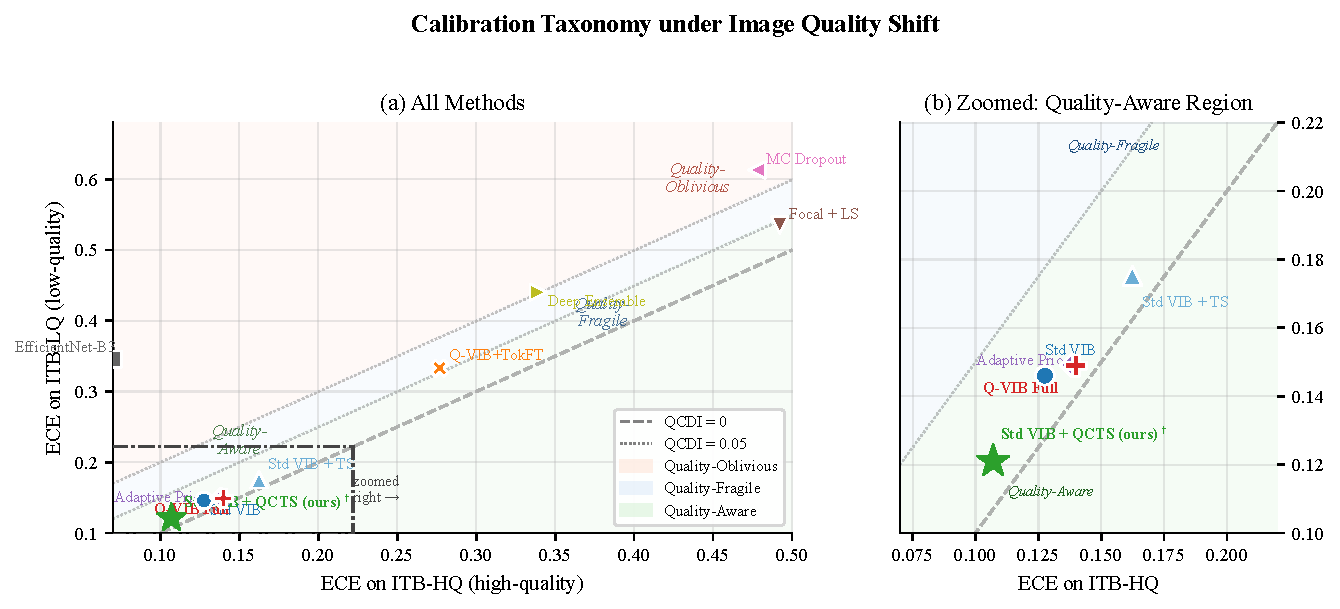
\includegraphics[width=\linewidth]{figures/fig1_taxonomy.pdf}
\caption{\textbf{Taxonomy scatter: ECE on ITB-HQ vs.\ ITB-LQ.} Distance above
  the diagonal equals QCDI; colour bands mark taxonomy class.
  D\,+\,QCTS and Q-VIB Full approach the $y{=}x$ (perfect invariance) line.}
\label{fig:scatter}
\end{figure}

Figure~\ref{fig:scatter} visualises the taxonomy. EfficientNet-B3
(QCDI\,=\,0.276) shows the starkest quality gap despite strong discriminative
performance. Standard TS (QCDI\,=\,0.013) appears Quality-Aware but its
positive $\rho$ ($+0.324$) reveals fundamentally oblivious behaviour---it
softens all predictions uniformly, destroying quality--confidence correlation.
Figure~\ref{fig:reliability} shows diverging reliability curves for
quality-oblivious methods vs.\ near-overlap for quality-aware ones.

\begin{figure}[htbp]
\centering
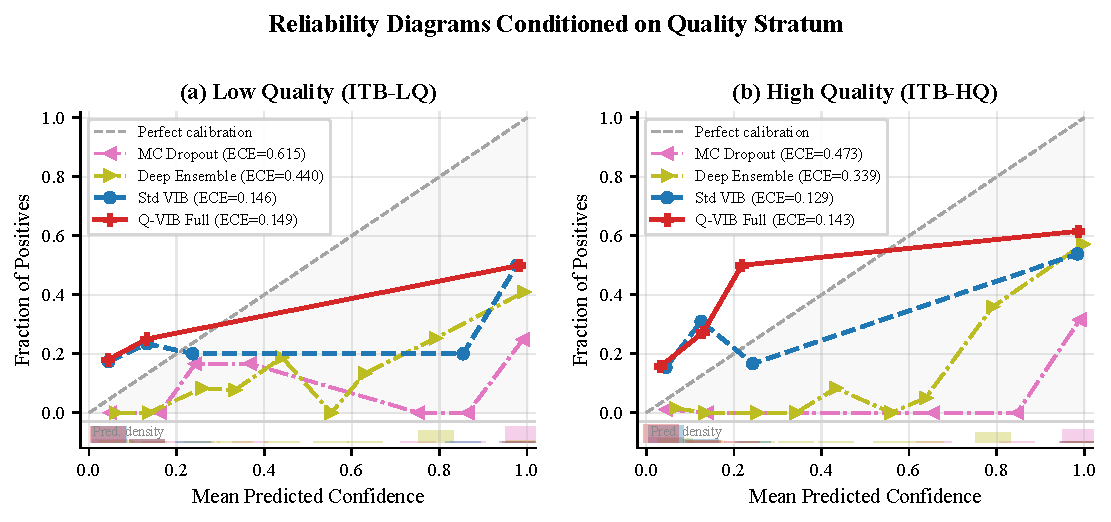
\includegraphics[width=\linewidth]{figures/fig2_reliability.pdf}
\caption{\textbf{Reliability diagrams conditioned on quality stratum.}
  Quality-oblivious methods (MC Dropout, Deep Ensemble) show diverging
  curves; quality-aware methods (Std VIB, Q-VIB Full) nearly overlap.}
\label{fig:reliability}
\end{figure}

\subsection{QCTS Analysis}
\label{sec:qcts_analysis}

\textbf{Effect on calibration.}
Applying QCTS to Std\,VIB reduces ITB-LQ ECE from 0.146 to 0.047 ($-$68\%),
improves $\rho$ from $-0.033$ to $-0.108$ (HAM10000), and transitions QCDI
from $+0.018$ to $-0.015$ (slight over-correction on LQ).
Figure~\ref{fig:tcurve} shows the learned $T(\qbar)$ across three seeds.

\textbf{Learned parameters.}
All three seeds converge to positive $\alpha$ (0.34, 0.96, 0.37), confirming
that quality-dependent modulation is robustly discovered. The optimisation
landscape has two apparent basins ($\alpha{\approx}0.35$ and $\alpha{\approx}0.96$);
the best run ($\alpha{=}0.96$, $T_0{=}1.17$) yields $T(\qbar{=}0){=}2.24$ vs.\
$T(\qbar{=}1){=}1.44$---temperature nearly doubles for worst-quality images.

\begin{figure}[htbp]
\centering
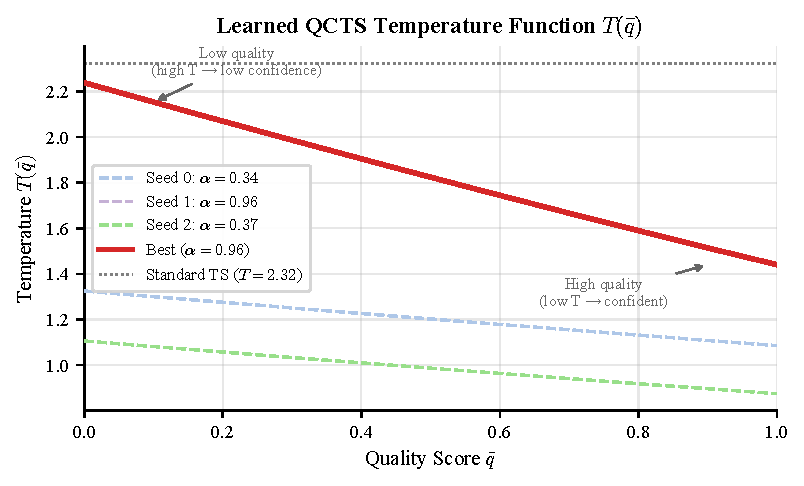
\includegraphics[width=0.85\linewidth]{figures/fig5_T_curve.pdf}
\caption{\textbf{Learned $T(\bar{q})$ across three seeds.} All converge to
  $\alpha{>}0$. Standard TS (horizontal dashed) is $\alpha{=}0$.}
\label{fig:tcurve}
\end{figure}

\textbf{Boundary condition: QCTS requires quality-sensitive representations.}
Applying QCTS to EfficientNet-B3 yields $\alpha{\approx}0$, recovering
standard TS. This null result is informative: QCTS amplifies quality-sensitive
signals already present in a model's logits. Purely discriminative models
produce logits uncorrelated with $\qbar$, leaving no signal to leverage. This
establishes a key boundary condition for post-hoc quality-aware calibration.

\textbf{Functional form ablation.}
We compare: (i)~softplus QCTS (proposed, QCDI\,=\,$-0.015$); (ii)~linear
$T(\qbar){=}\max(T_0{+}\alpha(1{-}\qbar), 0.1)$ (QCDI\,=\,$-0.004$); and
(iii)~piecewise-constant $T$ over $L{=}3$ quality bins
(QCDI\,=\,$+0.029$). Despite piecewise achieving the lowest validation NLL
(0.140 vs.\ softplus 0.152), it achieves the worst QCDI---demonstrating that
\emph{minimising NLL does not guarantee quality-aware calibration}. Smooth
interpolation across the quality spectrum is essential.

\subsection{Per-Degradation Analysis}

\begin{figure}[htbp]
\centering
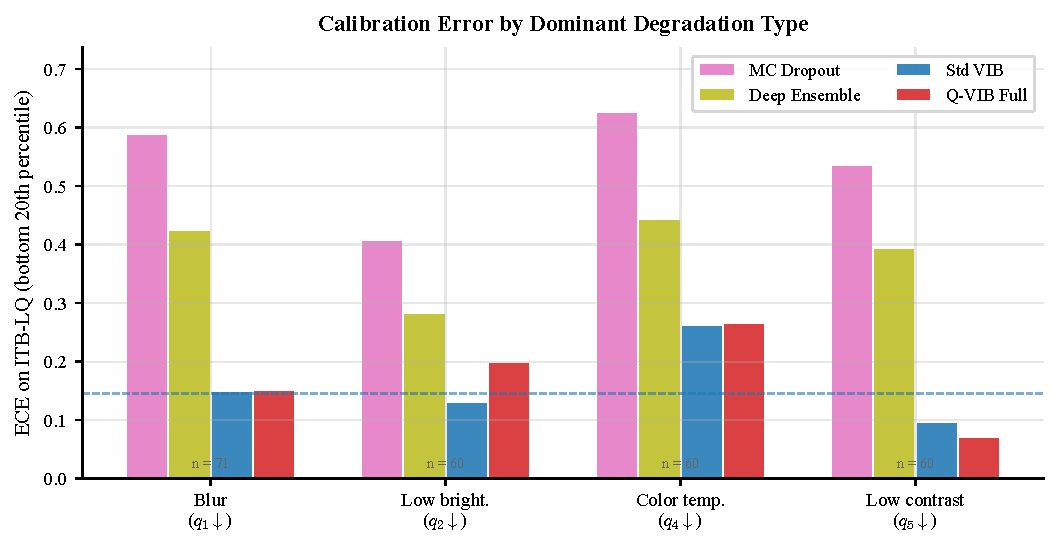
\includegraphics[width=\linewidth]{figures/fig3_degradation.pdf}
\caption{\textbf{ECE on ITB-LQ by degradation type} (bottom 20th percentile
  of each quality dimension). D\,+\,QCTS achieves the lowest ECE across three
  of four types.}
\label{fig:degradation}
\end{figure}

Not all degradations damage calibration equally (Table~\ref{tab:degradation},
Figure~\ref{fig:degradation}). \textbf{Colour temperature} ($q_4$) is the most
damaging across quality-oblivious methods (MC Dropout ECE\,=\,0.627), followed
by blur ($q_1$, ECE\,=\,0.590). Colour temperature shifts confound model confidence
in ways that misalign with accuracy, while blur---which destroys spatial detail---
has a slightly weaker effect. Low contrast ($q_5$) has the weakest impact on
Std\,VIB (ECE\,=\,0.056) and Q-VIB (0.057)---VIB models are sensitive to feature
magnitude rather than local contrast. D\,+\,QCTS achieves the lowest ECE across
three of four degradation types; Std\,VIB is optimal for low contrast where
QCTS over-corrects (0.088 vs.\ 0.056).

\begin{table}[htbp]
\centering
\caption{\textbf{Per-degradation ECE on ITB-LQ} (bottom 20th percentile of each quality
  dimension). Bold marks best per row.}
\label{tab:degradation}
\setlength{\tabcolsep}{4pt}
\footnotesize
\begin{tabular}{@{}lccccc@{}}
\toprule
Degradation & MC Drop. & DeepEns. & Std VIB & Q-VIB & \textbf{D+QCTS} \\
\midrule
Colour temp.\ ($q_4{\downarrow}$) & 0.627 & 0.443 & 0.264 & 0.266 & \textbf{0.155} \\
Blur ($q_1{\downarrow}$)          & 0.590 & 0.436 & 0.173 & 0.152 & \textbf{0.084} \\
Low brightness ($q_2{\downarrow}$)& 0.409 & 0.300 & 0.131 & 0.178 & \textbf{0.115} \\
Low contrast ($q_5{\downarrow}$)  & 0.538 & 0.430 & \textbf{0.056} & 0.057 & 0.088 \\
\bottomrule
\end{tabular}
\end{table}

\subsection{Cross-Dataset Generalization}

\begin{figure}[htbp]
\centering
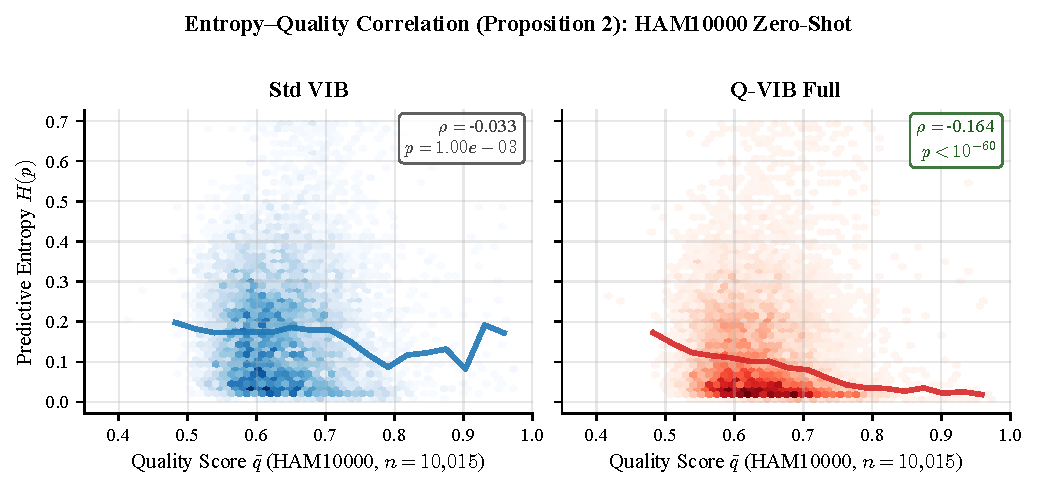
\includegraphics[width=\linewidth]{figures/fig4_entropy_qbar.pdf}
\caption{\textbf{Entropy vs.\ $\bar{q}$ on HAM10000 zero-shot} ($n{=}10{,}015$).
  Std VIB: near-zero correlation ($\rho{=}{-}0.033$). Q-VIB Full: strong
  negative trend ($\rho{=}{-}0.164$, $p{<}10^{-60}$).}
\label{fig:entropy}
\end{figure}

To test generalisability, we evaluate all methods zero-shot on HAM10000 and
PAD-UFES using VisiScore-Net quality scores
(Figure~\ref{fig:entropy}). Q-VIB Full maintains significantly negative
$\rho$ on both: $-0.164$ ($p{<}10^{-60}$, HAM10000) and $-0.236$
($p{<}10^{-29}$, PAD-UFES), consistent with ITB. QCDI rankings are
significantly correlated between ITB and HAM10000 (Kendall $\tau{=}0.71$,
$p{=}0.03$). The correlation with PAD-UFES is weaker ($\tau{=}{-}0.43$,
$p{=}0.24$), because PAD-UFES images are clinical-quality with limited quality
variation ($\qbar{>}0.45$ throughout), making absolute QCDI comparisons less
meaningful. The entropy-based $\rho$ metric, which does not require
stratification, shows consistent patterns across all three datasets.

%=====================================================================
\section{Discussion}
%=====================================================================

\textbf{Why do standard methods fail?}
MC Dropout and Deep Ensembles inject uncertainty at the \emph{parameter} level,
independent of input quality: a blurry image and a sharp one produce identical
dropout mask distributions. Temperature Scaling disproportionately softens large
logits typical of HQ inputs, raising entropy \emph{more} for high-quality
images---inverting the quality--confidence relationship ($\rho$: $-0.033
\to +0.324$). Both failure modes share a common root: no mechanism conditions
the predictive distribution on image quality. QCTS addresses this post-hoc by
learning $T(\qbar)$; Q-VIB addresses it architecturally. The QCTS--Q-VIB gap
($\Delta\rho{=}0.056$) quantifies the residual value of training-time
conditioning.

\textbf{Limitations and future work.}
ITB currently covers dermoscopy; extension to radiology or ophthalmology requires
modality-specific quality models. Programmatic degradation may not capture all
real-world artefacts (\eg specular reflections or inconsistent gel). QCTS
requires an external quality estimator, limiting applicability where none exists.
Translating reduced QCDI to improved clinical decision support requires
prospective evaluation.

%=====================================================================
\section{Conclusion}
%=====================================================================

We introduced Quality-Aware Calibration (QAC) and the Quality-Calibration
Degradation Index (QCDI) to formalise and measure how model calibration
degrades under image quality shift. Through the ITB benchmark---ten methods,
four quality-stratified subsets, four datasets---we demonstrated that widely-used
uncertainty methods are quality-oblivious despite their Bayesian motivation,
that standard Temperature Scaling actively inverts quality-awareness, and that
our proposed Quality-Conditioned Temperature Scaling (QCTS) reduces low-quality
ECE by 68\% post-hoc while the architecture-level Q-VIB remains the gold
standard. A key boundary condition emerges: post-hoc quality-aware calibration
requires the base model to carry quality-sensitive representations. We release
ITB and QCTS to facilitate systematic quality-aware evaluation of medical AI.

\bibliography{egbib}
\end{document}
